\section{Clasificación de los conjuntos numéricos}

Hasta aquí hemos trabajado con tres conjuntos numéricos relacionados entre sí:
\begin{itemize}
    \item \(\mathbb{N}\), los números naturales:
    \[
    0,1,2,3,\ldots
    \]
    \item \(\mathbb{Z}\), los números enteros, que incluyen a los naturales y a sus opuestos:
    \[
    \ldots,-3,-2,-1,0,1,2,3,\ldots
    \]
    \item \(\mathbb{Q}\), los números racionales, que pueden representarse mediante fracciones de enteros con denominador distinto de cero.
\end{itemize}

Como todo natural es entero y todo entero puede escribirse como una fracción con denominador \(1\), tenemos
\[
\boxed{\mathbb{N}\subseteq\mathbb{Z}\subseteq\mathbb{Q}}
\]

Por ejemplo,
\[
5=\frac51
\]
de modo que \(5\) es a la vez natural, entero y racional. Del mismo modo,
\[
-2=\frac{-2}{1}
\]
por lo que \(-2\) es entero y racional, pero no natural.

En la figura \ref{fig:jerarquia_numeros} se representan estas inclusiones mediante conjuntos anidados.

\begin{figure}[!ht]
  \centering
  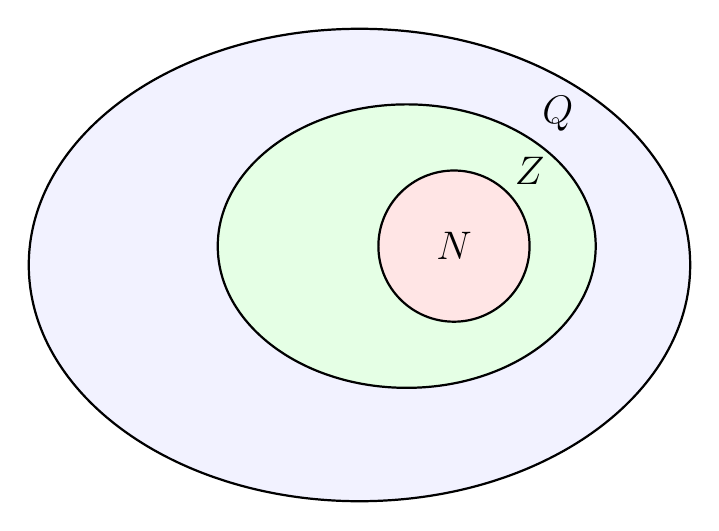
\begin{tikzpicture}[scale=1.2]
    % Elipse Q
    \draw[fill=blue!5,thick] (0,0) ellipse (3.5cm and 2.5cm);
    \node[font=\Large] at (2.1, 1.6) {\(\mathbb{Q}\)};
    
    % Elipse Z
    \draw[fill=green!10,thick] (0.5,0.2) ellipse (2cm and 1.5cm);
    \node[font=\Large] at (1.8, 1.0) {\(\mathbb{Z}\)};
    
    % Elipse N
    \draw[fill=red!10,thick] (1,0.2) ellipse (0.8cm and 0.8cm);
    \node[font=\Large] at (1, 0.2) {\(\mathbb{N}\)};
  \end{tikzpicture}
  \caption{Los números naturales están contenidos en los enteros, y los enteros están contenidos en los racionales.}
  \label{fig:jerarquia_numeros}
\end{figure}

Recuerde que la escritura decimal no constituye un nuevo conjunto numérico. Por ejemplo,
\[
0{,}5=\frac12
\]
por lo que \(0{,}5\) es un número racional.

